En esta sección analizamos primero generalidades sobre la planificación y luego entramos a ver en detalle el Sprint Backlog de cada iteración. A cada uno lo sigue un breve apartado sobre el seguimiento de la respectiva iteración, mostrando el burndown chart correspondiente. Finalmente realizamos la retrospectiva. 

\subsection{Comentarios preliminares sobre las User Stories}
\par Es un requerimiento que la comunidad sea la encargada de subir los bares. 
Sin embargo, es de esperar\footnote{En base a nuestra experiencia personal navegando por internet.} que los usuarios eventualmente agreguen bares repetidos, inexistentes, con información errónea o abusen del sistema de diversas formas (e.g. spam).
Consecuentemente, decidimos agregar un nivel de indirección, es decir que un usuario en vez de subir un nuevo bar, realiza una sugerencia a un Moderador (que puede aceptarla o rechazarla); éstos pueden ser miembros del equipo o usuarios distinguidos. 
Al verificar las sugerencias mediante un Moderador buscamos incrementar la calidad de los resultados.

\par El sistema de sugerencias a Moderadores se implementará no sólo para agregar nuevos bares, sino para modificar la información de bares ya existentes o para reconocer a los dueños de un bar.
Incorporamos el concepto de dueño de un bar, mediante el cual un usuario puede ser reconocido como propietario de un local, y puede actualizar la información del establecimiento sin requerir verificación de un Mod.

\par Ya que introducimos el concepto de Moderadores y de dueños de bares, algunos usuarios deben poder reconocerse.
Por ende, determinamos que los usuarios podrán tener una cuenta a la cual se loguean para utilizar ciertas funcionalidades de la aplicación.
Esto nos presentó un dilema: cómo tratar a los usuarios que no tienen cuentas?
Propusimos tres soluciones básicas: forzar a los usuarios a crear una cuenta y loguearse a ésta para utilizar la aplicación; permitir que los usuarios utilicen la aplicación ``deslogueados'', y que se logueen a sus cuentas para acceder a las funcionalidades que lo requieran; loguear automáticamente a los usuarios no registrados a una cuenta default (e.g. ``Guest'' o ``Anónimo''), y que se logueen para acceder a las funcionalidades correspondientes.

\par La primera opción nos pareció poco recomendable: las aplicaciones que requieren crear cuentas inmediatamente sin razón son molestas, y preferimos que los usuarios puedan usar la plataforma sin tener que loguearse.
Las otras dos opciones son esencialmente idénticas para el usuario; sin embargo, la tercera nos permite simplificar el código ya que podemos asumir que los usuarios siempre están logueados a una cuenta. 
Debido a esto, fue la que elegimos.

\par Para las features de los bares (e.g. calidad del wi-fi, cantidad de enchufes, precio) decidimos emplear una calificación de 5 estrellas, con una granularidad de media estrella\footnote{Las calificaciones posibles son $\{ \frac{1}{2}, 1, \frac{3}{2}, 2, \frac{5}{2}, 3, \frac{7}{2}, 4, \frac{9}{2}, 5 \}$.}.
Tener sólo 5 calificaciones posibles nos pareció muy restrictivo, por lo que adoptamos una granularidad de media estrella.
Discutimos sobre tomar 0 o media estrella como calificación mínima; decidimos adoptar media por claridad, pues una valoración de 0 estrellas puede ser confundida con que nadie haya calificado aún la feature.

\par En lo que concierne a la presentación de los bares más cercanos, decidimos ordenarlos siempre por distancia.
Adicionalmente, el usuario puede aplicar filtros por feature, eliminando resultados que no cumplen ciertos criterios. 
Éstos pueden ser, $\leqslant, \geqslant$, o por rango cerrado (e.g. si la calificación $\in [2, 4]$)\footnote{Para algunas features, como precio, se podrán utilizar todos estos filtros; para otras, sólo algunos: no tiene sentido buscar sólo bares con mala calidad de wi-fi.}.

\par La User Story a la que le asignamos 1 Story Point es a ``Borrar Comentarios'', ya que consiste sólo en agregar un botón a la interfaz de comentarios y removerlo de la estructura que lo contiene, ambas tareas muy sencillas. Para decidir el resto de los Story Points de los User Stories utilizamos la técnica de Planning Poker.

\subsection{Roles de usuario}
\par Consideramos que la siguiente elección de roles nos da una granularidad suficiente para nuestro problema:

\begin{itemize}
  \item usuario que busca un bar: un usuario cuyo objetivo es encontrar un bar.
  \item usuario que critica un bar: un usuario que quiere criticar un bar, lo cual puede hacerlo a través de comentarios y calificaciones.
  \item usuario con cuenta y usuario sin cuenta: son respectivamente los roles para usuarios que están o no registrados, y que realizan acciones relacionadas a este sistema de registro.
  \item moderador: usuario con privilegios especiales que le permiten agregar, editar y eliminar todos los bares.
  \item dueño de bar: usuario con privilegios especiales para editar o eliminar el o los bares que posee.
  \item usuario que usa Facebook y usuario que usa Twitter: son los roles asociados a la interacción con redes sociales.
\end{itemize}

%%%%%% PRIMER SPRINT %%%%%%
\subsection{Primer Sprint: Sprint Backlog}
\par Para el primer Sprint elegimos las User Stories esenciales para implementar la funcionalidad básica de buscar un bar cercano: la búsqueda en sí, la vista de bares y sus features, agregar bares (sólo como Moderador, ya que es más simple y con esto alcanza en una primera instancia), el log-in\footnote{Si bien podremos loguearnos a cuentas ya existentes, aún no podremos crear nuevas. Hardcodearemos algunas, y nos loguearemos a éstas.} y la promoción a Moderador.
Estas dos últimas son necesarias ya que un bar sólo puede ser agregado por un Moderador.

\subsubsection*{Buscar bares}
  \userstory{usuario que busca un bar}{buscar bares cerca de mí}{poder conocer qué bares cercanos tienen wifi y enchufes.}
  \critdeacep{Al enviar la posición actual del usuario al sistema, este debe devolver la lista de bares a menos de 400m.}
  \valores{10}{8}{1.25}
  \tasks{
    \begin{enumerate}
      \item Crear página de búsqueda. (2)
      \item Crear la función de búsqueda, que toma como parámetro la posición del usuario. (3)
      \item Devolver una lista de jsons para cada bar con su nombre, su distancia, su valoración y un link a su página dentro de la aplicación. (1)
      \item[] \textit{Total de horas hombre:} 6
    \end{enumerate}
  }

\subsubsection*{Agregar bares}
  \userstory{moderador}{poder agregar un nuevo bar}{que pueda ser sugerido por la aplicación a los usuarios}
  \critdeacep{El moderador debe poder cargar los datos y crear un bar. El bar debe aparecer en las búsquedas posteriores, reflejando su existencia en el sistema.}
  \valores{8}{5}{1.6}
  \tasks{
    \begin{enumerate}
      \item Añadir botón en el menú de acciones del moderador para agregar a la base de datos un nuevo bar. (1)
      \item Hacer que al presionar un botón se cargue un formulario para rellenar con los datos del bar. (3)
      \item Hacer una función que dado un formulario cree una entrada en la base de datos. (2)
      \item[] \textit{Total de horas hombre:} 6
    \end{enumerate}
  }

\subsubsection*{Borrar bares}
  \userstory{moderador o dueño del bar}{poder borrar un bar existente}{que no pueda ser sugerido por la aplicación a los usuarios}
  \critdeacep{Un bar del catálogo debe poder ser seleccionado por el moderador o el dueño del bar. Si un usuario busca el bar eliminado, éste no deberá aparecer. Si un usuario está puntuando o comentando cuando se elimina, recibirá un error. Si dos moderadores intentan borrar simultáneamente el mismo bar, el último en hacerlo recibirá un error.}
  \valores{5}{2}{2.5}
  \tasks{
    \begin{enumerate}
      \item Agregar botón en la página del bar para que pueda ser borrado por un moderador o su dueño. (2)
      \item Hacer una función que lo elimine de la base de datos. (1)
      \item[] \textit{Total de horas hombre:} 3
    \end{enumerate}
  }

\subsubsection*{Vista del bar}
  \userstory{usuario que busca o critica un bar}{poder acceder a la página de un bar en la aplicación}{ver sus características con mayor detalle}
  \critdeacep{La vista del bar debe contener todos los datos actualizados: nombre, foto, ubicación, features y comentarios.}
  \valores{10}{3}{3.33}
  \tasks{
    \begin{enumerate}
      \item Agregar un template para la página correspondiente a la vista de un bar. (3)
      \item Agregar una función para traer los datos actualizados del bar en un json desde la base de datos. (1)
      \item[] \textit{Total de horas hombre:} 4
    \end{enumerate}
  }

\subsubsection*{Log-in}
  \userstory{usuario con cuenta}{loguearme}{acceder a funcionalidades disponibles sólo a usuarios con cuenta.}
  \critdeacep{Al ingresar un usuario y contraseña válidas, el sistema debe iniciar una sesión con ese usuario.}
  \valores{8}{5}{1.6}
  \tasks{
    \begin{enumerate}
      \item Crear un sistema de log-in. (3)
      \item Crear una página de log-in para que los usuarios puedan ingresar su usuario y contraseña. (2)
      \item[] \textit{Total de horas hombre:} 5
    \end{enumerate}
  }

\subsubsection*{Promover a moderador}
  \userstory{moderador}{dar privilegios de moderación a un usuario con cuenta}{permitir que un usuario confiable pueda ser moderador.}
  \critdeacep{Si el usuario seleccionado existe, se le deberán otorgar privilegios de moderación y tendrá disponibles todas las herramientas de los moderadores a partir de ese momento.}
  \valores{5}{3}{1.66}
  \tasks{
    \begin{enumerate}
      \item Hacer función que le de privilegios de moderación a una cuenta. (1)
      \item[] \textit{Total de horas hombre:} 1
    \end{enumerate}
  }

\subsection{Primer Sprint: Seguimiento}

\begin{figure}[H]
 \centering
  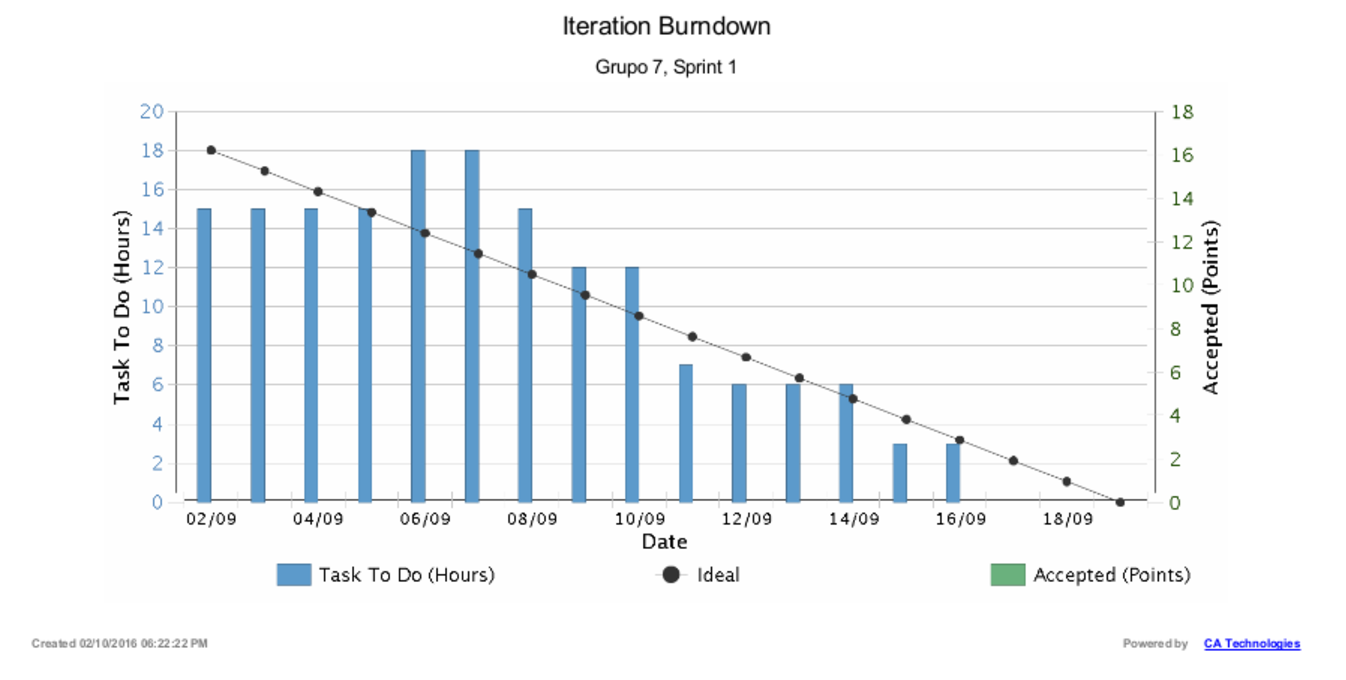
\includegraphics[width=\textwidth]{diagramas/iteration_burndown1.pdf}
  \caption{}
  \label{fig:burndown1}
\end{figure}

La subida en la cantidad de horas restantes que puede observarse el 06/09 se explica porque se nos había pasado por alto asignarle la estimación de horas a la User Story ``Vista de bar'' al momento de crearla. El 06/09 fue cuando corregimos dicho error.

En general quedamos muy conformes con el flujo de trabajo durante este primer sprint. Como puede verse en el gráfico logramos mantenernos al día, cumpliendo con todos los objetivos propuestos.

%%%%%% SEGUNDO SPRINT %%%%%%
\subsection{Segundo Sprint: Sprint Backlog}
\par En el segundo Sprint buscamos expandir significativamente el proceso de búsqueda y vista de bares, incorporando filtros por feature y distancia, permitiendo editar información de bares (nuevamente, sólo como Moderador), calificarlos, comentar y obtener el trayecto óptimo hasta el bar.
También agregaremos la opción de crear cuentas, ya que la alternativa de hardcodearlas es engorrosa.


\subsubsection*{Editar información de bares}
  \userstory{moderador o dueño del bar}{poder editar la información de un bar del sistema}{actualizar datos incompletos, incorrectos o desactualizados.
  }
  \critdeacep{Dado un bar, el dueño o un moderador debe tener un botón para editarlo dentro de la página del bar. Luego de editarlo, si alguien accede la página del bar, éste aparecerá con sus datos actualizados. Si dos moderadores editan un bar al mismo tiempo, la edición definitiva será la del que lo envíe segundo.}
  \valores{6}{3}{2}
  \tasks{
    \begin{enumerate}
      \item Agregar botón en el menú de acciones que tiene el moderador/dueño del bar sobre cada bar para que pueda editar la información. (1)
      \item Hacer que al presionar el botón se cargue un formulario con la información actual del bar, la cual podrá ser editada y actualizada en la base de datos al presionar un botón de confirmación. (4)
      \item[] \textit{Total de horas hombre:} 5
    \end{enumerate}
  }

\subsubsection*{Votación}
  \userstory{usuario que critica un bar}{poder calificar a un bar con una cantidad de estrellas del $\frac{1}{2}$ (peor) al $5$ (mejor) en todas sus features}{dar una valoración rápida y concreta que ayude al resto de la comunidad en sus futuras búsquedas.}
  \critdeacep{Cuando un bar es calificado por un usuario, el nuevo voto deberá verse reflejado cuando la página del bar sea cargada posteriormente.}
  \valores{9}{2}{4.5}
  \tasks{
    \begin{enumerate}
      \item Modificar la representación de los bares para que pueda almacenar el promedio de votos de cada categoria y la cantidad de votos de cada categoria. (2)
      \item Hacer que las funciones que leen la información de un bar lean también las calificaciones. (2)
      \item[] \textit{Total de horas hombre:} 4
    \end{enumerate}
  }

\subsubsection*{Comentar}
  \userstory{usuario que critica un bar}{escribir comentarios sobre los bares que visito}{compartir detalles que considere importantes para ayudar al resto de la comunidad en futuras búsquedas.}
  \critdeacep{Al escribir y aceptar un nuevo comentario, éste debe aparecer en la vista del bar.}
  \valores{7}{2}{4.5}
  \tasks{
    \begin{enumerate}
      \item Modificar la representación de los bares para que pueda almacenar una lista de comentarios. (1)
      \item Modificar la página de vista de los bares para que puedan mostrarse los últimos 10 comentarios. (2)
      \item Agregar un botón para que puedan verse todos los comentarios de un bar. (2)
      \item[] \textit{Total de horas hombre:} 5
    \end{enumerate}
  }

\subsubsection*{?`Cómo llegar?}
  \userstory{usuario que busca un bar}{conocer la ruta más rápida para llegar al bar deseado desde mi posición actual}{minimizar mi pérdida de tiempo y esfuerzo.}
  \critdeacep{En la vista de un bar deberá haber un botón que permita ver el camino al bar desde mi posición. Éste deberá ser efectivamente el camino óptimo.}
  \valores{9}{3}{3}
  \tasks{
    \begin{enumerate}
      \item Agregar un botón en la vista de un bar que permita acceder al mapa de camino más rápido. (1)
      \item Interactuar con la API de Google Maps para obtener el mapa. (3)
      \item[] \textit{Total de horas hombre:} 4
    \end{enumerate}
  }


\subsubsection*{Filtrar por distancia}
  \userstory{usuario que busca un bar}{filtrar los resultados de una búsqueda de bares por máxima distancia}{buscar y distinguir bares según la distancia a la que se encuentran}
  \critdeacep{Al modificar la preferencia de distancia máxima de búsqueda, los bares resultantes deberán encontrarse a menor o igual distancia que la seleccionada.}
  \valores{8}{2}{4}
  \tasks{
    \begin{enumerate}
      \item Agregar opción de filtro por distancia a la lista de resultados. (1)
      \item Agregar función de filtrado por distancia y filtrar los resultados usándola. (3)
      \item[] \textit{Total de horas hombre:} 4
    \end{enumerate}
  }

\subsubsection*{Filtrar búsquedas por feature}
  \userstory{usuario que busca un bar}{filtrar los resultados de una búsqueda según el puntaje de las distintas features de los bares}{poder descartar de los resultados los bares que tengan una puntuación indeseable en ciertas categorías}
  \critdeacep{Al seleccionar un filtro, los resultados de la búsqueda ejecutada que aparecen deben pasar las condiciones impuestas por los filtros, y deben ser todos los que las cumplen.}
  \valores{8}{3}{2.66}
  \tasks{
    \begin{enumerate}
      \item Hacer función que chequee si un bar pasa los criterios especificados. (2)
      \item Filtrar los resultados que se le muestran al usuario utilizando dicha función. (2)
      \item[] \textit{Total de horas hombre:} 4
    \end{enumerate}
  }

\subsubsection*{Creación de cuenta}
  \userstory{usuario sin cuenta}{crear una cuenta}{poder loguearme y acceder a funcionalidades sólo disponibles a usuarios logueados.}
  \critdeacep{Al ingresar un usuario y contraseña y confirmar la contraseña, si el usuario no existe en el sistema, se creará un nuevo usuario, que podrá loguearse de ahí en adelante.}
  \valores{9}{3}{3}
  \tasks{
    \begin{enumerate}
      \item Hacer una página de creación de usuarios. (1)
      \item Hacer función que cree usuario. (1)
      \item[] \textit{Total de horas hombre:} 2
    \end{enumerate}
  }

\subsection{Segundo Sprint: Seguimiento}

\begin{figure}[H]
 \centering
  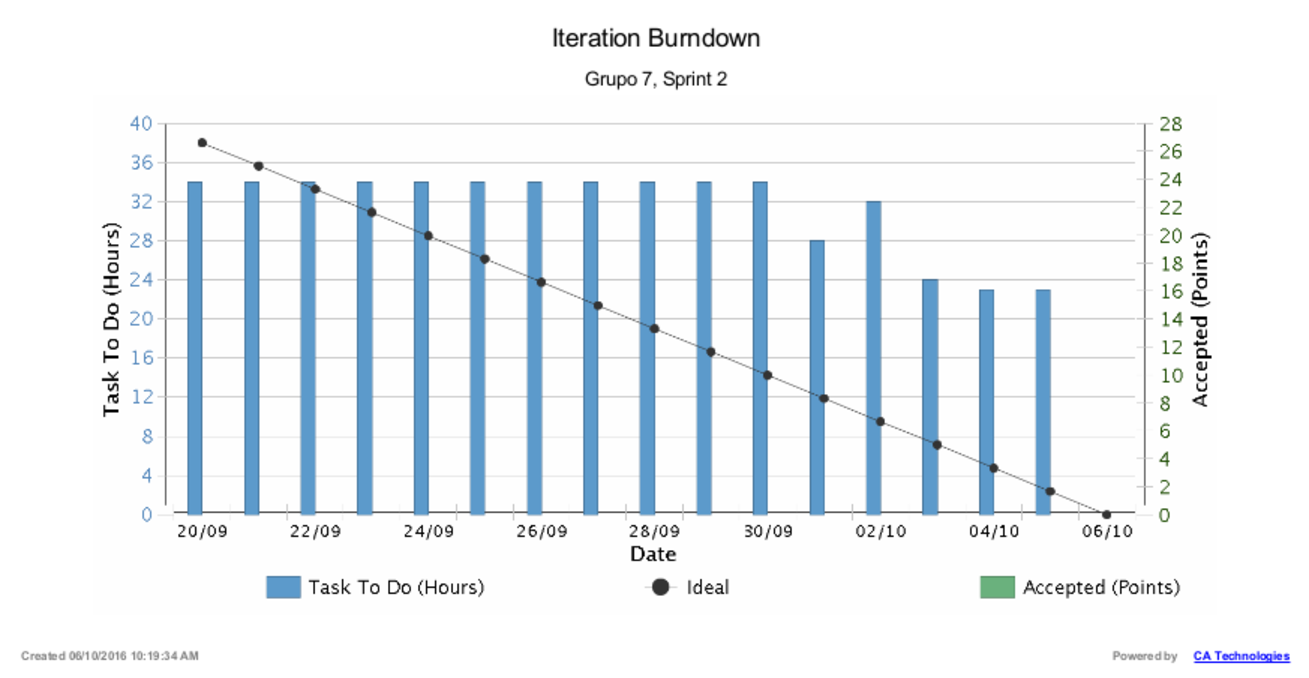
\includegraphics[width=\textwidth]{diagramas/iteration_burndown2.pdf}
  \caption{}
  \label{fig:burndown2}
\end{figure}

A diferencia del primer sprint, el flujo de trabajo que muestra el gráfico no es demasiado satisfactorio. Pasamos mucho tiempo antes de empezar a bajar las horas de trabajo pendientes. Esto se debió en parte a una mayor carga de trabajo con respecto al primer sprint, pues la intención era aumentar nuestra \emph{velocity}, habida cuenta que nuestro conocimiento del problema era mayor tras realizar la primer iteración. Sin embargo, no ponderamos lo suficiente otros factores externos, como una mayor demanda de la Facultad dado que era época de parciales y entregas de otras materias.

No obstante a esto, logramos recuperarnos y llevar a cabo el trabajo propuesto para este sprint.

%%%%%% FUTUROS SPRINTS
\subsection{Retrospectiva}
\par Si bien en estas dos primeras iteraciones del proyecto pudimos desarrollar el núcleo de las funcionalidades relacionadas con la búsqueda de bares, la aplicación aún dista mucho de estar completamente terminada. Quedan un gran número de cosas por hacer:
\begin{itemize}
 \item algunas que son claves pues hacen a los requerimientos iniciales de la aplicación, como por ejemplo que los usuarios puedan sugerir nuevos bares; 
 \item otras que apuntan más a un refinamiento de lo que ya hay, como hacer más cómoda la búsqueda de bares evitando que el usuario tenga que volver a buscar un bar cada vez que retorna de ver un perfil, o que los usuarios con cuenta tengan un historial de comentarios y calificaciones;
 \item y también extender la aplicación con otras funcionalidades (no centrales inicialmente) que pueden ser claves en la mecánica del negocio, como interactuar con redes sociales.
\end{itemize}

\par Además de esto, para la user story ``Votación'' del segundo sprint, tuvimos que realizar una ligera simplificación: en lugar de calificar con estrellas como habíamos explicado antes, decidimos calificar con números del 1 al 10. Este sistema nos resultó más rápido para implementar inicialmente y tiene la ventaja de que mantiene el mismo nivel de granularidad (en ambos casos hay 10 puntajes posibles). Sin embargo, como es un requerimiento del Product Owner que el voto se realice con estrellas, volveremos a poner ``Votación'' en el backlog, con el propósito de modificar esta cuestión

\par A continuación presentamos las User Stories que actualmente nos quedan en el backlog.

\subsubsection*{Votación}
  \userstory{usuario que critica un bar}{poder calificar a un bar con una cantidad de estrellas del $\frac{1}{2}$ (peor) al $5$ (mejor) en todas sus features}{dar una valoración rápida y concreta que ayude al resto de la comunidad en sus futuras búsquedas.}
  \critdeacep{Cuando un bar es calificado por un usuario, el nuevo voto deberá verse reflejado cuando la página del bar sea cargada posteriormente.}
  \tasks{
    \begin{enumerate}
      \item Backend: Adaptar el sistema de votos actual para que en lugar de usar un número del 1 al 10 utilice una cantidad de estrellas del 1 al 5 con granularidad $\frac{1}{2}$ (1)
      \item Frontend: Que cada \emph{feature} para votar tenga una barra de 5 estrellas que permita seleccionar el puntaje deseado con el mouse, y que se lo comunique a el backend (3)
      \item[] \textit{Total de horas hombre:} 4
    \end{enumerate}
  }

\subsubsection*{Volver a página de resultados}
  \userstory{usuario de la aplicación}{poder volver a los resultados obtenidos en una búsqueda desde la vista de un bar seleccionado a partir de la misma}{poder acceder a las vistas de otros bares obtenidos en la búsqueda sin tener que volver a realizarla}
  \valores{5}{3}{1.66}

\subsubsection*{Sugerir un nuevo bar}
  \userstory{usuario con cuenta}{sugerir que se agregue un nuevo bar}{que pueda ser aprobado por un mod y de esta forma sea agregado al catálogo}
  \valores{7}{5}{1.4}

\subsubsection*{Sugerir dueño de un bar}
  \userstory{usuario con cuenta}{proponerme como dueño de un bar que ya se encuentra en el sistema}{ser reconocido como dueño del bar y poder actualizar su información libremente.}
  \valores{5}{5}{1}

\subsubsection*{Aprobar la creación de un bar}
  \userstory{moderador}{poder aprobar o rechazar una sugerencia para agregar un nuevo bar}{para que la sugerencia sea procesada y removida de la cola.}
  \valores{5}{5}{1}

\subsubsection*{Aprobar dueño}
  \userstory{moderador}{poder aprobar o rechazar la sugerencia de un usuario que se indica como dueño de un bar}{para que la sugerencia sea procesada y removida de la cola.}
  \valores{5}{5}{1}

\subsubsection*{Remover comentarios}
  \userstory{moderador}{remover comentarios}{hacer cumplir las condiciones de uso de la aplicación.}
  \valores{3}{1}{3}

\subsubsection*{Interactuar con Facebook}
  \userstory{usuario que usa Facebook}{compartir el perfil del bar en mi muro de Facebook}{mis contactos de Facebook conozcan el bar y sepan mi opinión al respecto.}

\subsubsection*{Interactuar con Twitter}
  \userstory{usuario que usa Twitter}{twittear el perfil del bar}{mis contactos de Twitter conozcan el bar y sepan mi opinión al respecto.}

\subsection{Modificaciones respecto de la primer entrega}
Se realizaron las siguientes modificaciones menores a partir de las correcciones recibidas tras la primer entrega de las user stories:
\begin{itemize}
  \item Tratamos de ser más realistas en cuanto a lo que falta por hacer, no dar ``la sensación de tener toda la aplicación terminada en dos sprints''.
  \item Pasamos de tener un único rol genérico para los usuarios a varios más específicos.
  \item Agregamos al backlog User Stories relacionadas con la interacción con redes sociales. 
\end{itemize}